% compiler: XeLaTeX
\documentclass[a4paper, AutoFakeBold]{article}
\usepackage{graphicx}
\usepackage[a4paper,top=2.54cm,bottom=2.54cm,left=2.7cm,right=2.7cm]{geometry}

% 载入常用的数学包, 符号包
\usepackage{amsmath}
\usepackage{mathtools}
\usepackage{amsfonts}
\usepackage{amssymb}
\usepackage{mathrsfs}
\usepackage[justification=centering]{caption}
\usepackage[bookmarks=true,colorlinks=true,linkcolor=magenta,citecolor=blue,urlcolor=magenta]{hyperref}
\usepackage{booktabs}
\usepackage{blindtext}
\usepackage{calc} % 用于使用宽度和长度的计算

%% linespace 行间距,段间距等等
\usepackage{setspace}

\setlength{\parindent}{2em}
\fontsize{12pt}{15pt}\selectfont    % 小四号,1.25倍行距
% fonts (style, color, size).
\usepackage{ctex}		 	% If you are lazy, the CTEX suit is enough.

% Chinese font
\usepackage{xeCJK}		 	% For the Chinese through XeLaTex
\setCJKmainfont{SimHei.ttf} 	% set the mainfont of Chinese as songti. (serif) for
\setCJKsansfont{SimHei.ttf}	% sans serif font for \textsf
\setCJKmonofont{SimHei.ttf}	% monospace font for \texttt
% \punctstyle{kaiming}   	% Remove the space used by symbols like comma.
\setCJKfamilyfont{song}{SimSun.ttf}
\newcommand{\song}{\CJKfamily{song}} %宋体 song
\setCJKfamilyfont{kai}{SimKai.ttf}
\newcommand{\kai}{\CJKfamily{kai}} %楷体2312  kai
\setCJKfamilyfont{hei}{SimHei.ttf}
\newcommand{\hei}{\CJKfamily{hei}} %黑体  hei

% English font
\usepackage{fontspec}
\setmainfont{Times New Roman}
\setsansfont{Times New Roman}
\setmonofont{Times New Roman}
% font Size
\newcommand{\yihao}{\fontsize{26pt}{18pt}\selectfont}
\newcommand{\erhao}{\fontsize{22pt}{18pt}\selectfont}
\newcommand{\xiaoerhao}{\fontsize{18pt}{18pt}\selectfont}
\newcommand{\sanhao}{\fontsize{16pt}{18pt}\selectfont}
\newcommand{\sihao}{\fontsize{14pt}{17.5pt}\selectfont}
\newcommand{\xiaosihao}{\fontsize{12pt}{15pt}\selectfont}
\newcommand{\wuhao}{\fontsize{10.5pt}{13.125pt}\selectfont}


% set the styles of sections at all levels
\usepackage{titlesec}
\usepackage{titletoc}
\titleformat{\section}{\hei\bfseries\sihao}{\thesection.}{1em}{} % 在section标题编号后面加个点
\titleformat{\subsection}{\raggedright\hei\bfseries\xiaosihao}{\thesubsection.}{1em}{}
\titleformat*{\subsubsection}{\raggedright\hei\bfseries\xiaosihao}
\titleformat{\paragraph}[hang]{\raggedright\hei\bfseries\xiaosihao}{\theparagraph}{1em}{}[]

\usepackage{abstract} % 引入abstract宏包

% 设置摘要的格式
\renewenvironment{abstract}%
  {% 开始
    \begin{center}%
    \bfseries % 加粗
    \erhao % 字体大小
    \thetitle % 显示"摘要"标题
    \end{center}%
    \par
    \xiaosihao
    \noindent
    \textbf{摘要:}
  }%
  {% 结束
    \par
    \vspace{1em}
    \noindent
    \textbf{关键词:} % 显示"关键词:"标题
  }
\newcommand{\keywords}[1]{\xiaosihao #1}


% reference and citation 参考文献
\usepackage[numbers]{natbib}
\renewcommand{\refname}{\hei\sihao \centerline{参考文献}\vspace{-1em}}
\bibsep=0pt % 用来设置每个\bibitem之间的间距
% \newcommand{\upcite}[1]{\textsuperscript{\textsuperscript{\cite{#1}}}} % show citation label in the upperscript

\usepackage{listings} % For the code. 代码
\usepackage{appendix}
\renewcommand{\appendixname}{附录}

% titlepage
\usepackage{titling}
% 重置命令 maketitle
\renewcommand{\maketitle}{
	\def\titlelength{8em}
 	\begin{titlepage}
		\begin{center}
			\vspace*{2em}
            {\sihao \hei 中国科学院大学人工智能学院《文献阅读》课程—文献综述报告}\\
            \vspace*{-0.5em}
            \rule{\textwidth}{0.5pt}\\
			\vspace*{3em}
			{\sihao \hei \bfseries 课程编号:}
            {\sihao \courseID}\\
			\vspace*{11em}
			{\yihao \hei \bfseries \thetitle}

			\vspace*{9em}
			{\sanhao \hei
				\renewcommand\arraystretch{1.5}
				\begin{tabular}{ll}
					\makebox[4em][r]{{\bfseries 撰写人:}} &
					\makebox[\titlelength][l]{\theauthor} \\
					\makebox[4em][r]{{\bfseries 学号:}} &
					\makebox[\titlelength][l]{\studentID} \\
					\makebox[4em][r]{{\bfseries 培养单位:}} &
					\makebox[\titlelength][l]{\organization} \\
			  \end{tabular}
		    }

			\vspace{4em}
			{\sanhao \bfseries \thedate}
		\end{center}
	\end{titlepage}
}


\newcommand{\mytitle}{时序知识图推理方法研究}
\title{\mytitle}
\author{宋超}
\def\courseID{180206081104P3012H-01}
\def\studentID{202328020629002}
\def\organization{中国科学院自动化研究所}
\date{\today}

\begin{document}

\maketitle

% \clearpage
\setcounter{page}{1}
\begin{abstract}
自知识图谱(Knowledge Graph, KG)的概念提出以来,各大企业、机构纷纷利用知识图谱构建了庞大的知识库(Knowledge Base, KB)。但是由于知识库的不完备性,如何利用已有知识预测缺失的知识,从而完善知识库这个问题被提了出来,进而出现了知识图完备(Knowledge Graph Completion, KGC)相关的研究。然而现实世界中的知识往往不是一成不变的,于是近年来又出现了带时间信息的知识库(Temporal Knowledge Base, TKB),以及相应的时序知识图完备\cite{2023survey}(Temporal Knowledge Graph Completion, TKGC,或称时序知识图推理\cite{7-2021} Temporal Knowledge Graph Reasoning,TKGR)相关的研究。本文通过调研目前主流的研究方法与分类方式,选择了我们认为具有代表性的三个框架 TLogic, MPNet, ECEformer 来介绍当前 TKGC 的最新进展。
\end{abstract}
\keywords{文献综述;时序马尔可夫逻辑网络;时序知识图谱;时序知识图完备;时序知识图推理}

\section{简介}

在马尔可夫逻辑网络(Markov Logic Network, MLN)出现之前,符号主义者们提出一阶谓词逻辑(First Order Logic)来对知识进行表示和推理,但是它不具备处理不确定性的能力;另一种方法是概率图模型(Probabilistic Graphical Model),它引入概率来处理不确定性,但是在知识的表示和推理方面存在不足。MLN 的出现将两者结合在一起,它为一阶知识库里的每个公式(formula)赋予权重,这个权重可以通过迭代优化学习得到,然后再使用马尔可夫链-蒙特卡罗方法\cite{20-1996}(Markov Chain Monte Carlo,MCMC)就可以实现对具体请求的推理\cite{2006mln}。MLN 的出现极大地推动了相关研究的发展,包括知识图谱概念的提出\cite{8-2024},并且对很多后续方法起到了奠基作用。

然而 MLN 所表达的世界有一个严重的缺陷——它所描述的世界是静态的,现实世界中很多知识却都是有时效的,比如“美国的总统是拜登”在某些年份里可能是对的,在其它时间里就是错的。在解决静态 KGC 问题中,尝试通过利用知识库中的事实规则进行推理的方法被称为基于规则的方法,到了 TKGC 问题中,将这些规则与时间信息相结合也可以取得良好的效果,其中一些方法尝试通过先学习一些静态规则,然后再为其赋予时间特征,如 StreamLearner\cite{11-2019};另一种思路是通过随机游走的方法加上时间约束,以此来得到包含时序信息的规则,进而进行推理。使用随机游走的方法中,TLogic\cite{3-2022}是第一个直接从 TKG 中学习时序规则并将其应用于推理中的方法,我将在后文中展开介绍此方法。
随着人工神经网络的发展,除了使用基于规则的,人工神经网络(Neural Network)也被用来进行 TKGC 的研究,并取得了良好的效果。其中,把知识图中的实体和关系表示为词嵌入形式,然后将时间信息按照先后顺序、或者作为属性放入人工神经网络中训练,最后使用训练得到的模型对给定的查询进行推理,这类方法被称为知识图嵌入(Knowledge Graph Embedding,KGE)方法,如 DArtNet\cite{5-2020},ComplEx\cite{21-2016}。另外还有基于强化学习的方法,如MPNet\cite{4-2024}。还有使用 encoder-decoder 架构分别获得 TKG 的全局与局部特征然后将它们用于链路预测的RE-Net\cite{12-2020},使用 attention 机制实现的ECEformer\cite{6-2024}。



\begin{figure}
	\captionsetup{width=0.8\textwidth}
	\centering
	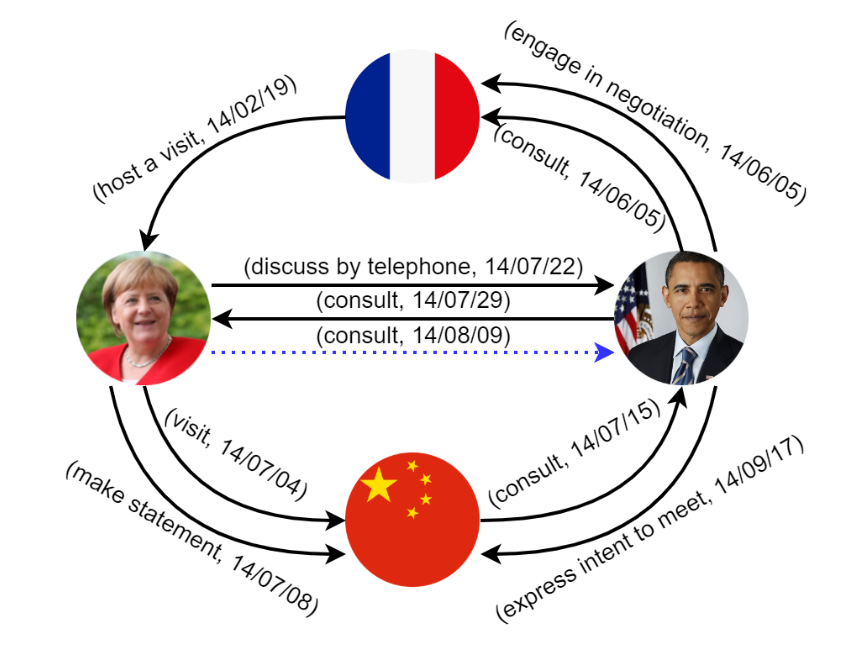
\includegraphics[width=0.5\textwidth]{figures/TKG.png}
	\caption{时序知识图谱实例,取自 ICEWS14 的一个子图,其中 Angela Merkel, Barack Obama, France 和 China 是实体,时间以 yy/mm/dd 的形式表示。蓝色的虚线构成查询 (Angela Merkel, consult, ?, 2014/08/09) 的答案。\cite{3-2022}}
\end{figure}



从分类上看,目前用于 TKGC 的方法可以从两个维度进行分类:
第一种分类方式通过算法所属的机器学习方法阵营进行分类,可分为符号主义型方法、联结主义型方法和行为主义型方法。符号主义侧重于从 TKG 中找到可信的规则,然后应用这些规则进行时序推理,其优点是可以发掘图中的固有逻辑信息,而且具有可读可解释性,这类方法占比不多,但效果不俗,其中比较有代表性的是 TLogic,它通过随机游走的方式从时序知识图中探索规则,然后将规则应用于查询对象,结合历史事实对缺失实体进行预测。由于人工神经网络近年来大放光彩,多数方法还是基于人工神经网络的方法,属于联结主义阵营。这类方法使用循环神经网络RNN来学习时序知识图的时序信息,使用图神经网络GNN来学习时序图中的结构信息。这类方法可以单独使用RNN,如 DArtNet\cite{5-2020} 和 RE-Net\cite{12-2020},或者使用 RNN 的同时再结合 GNN,如 RE-GCN\cite{7-2021}。在各类机器学习任务中取得良好效果的 Transformer 也有在此方面的应用,如 ECEformer\cite{6-2024}。而行为主义型方法主要是基于强化学习的方法,如 MPNet\cite{4-2024}。
另一种分类方法着眼于方法对 TKG 中信息挖掘的侧重点,分为“内插法”与“外推法”两类。简单而言,内插法预测的时间范围不会超过训练集自身的时间范围,而外推法则会对发生在训练集时间范围之外的事件进行预测。从本质上来说,内插法侧重于用地图或几何的方法探索图中的结构与语义信息,而外推法则重在针对具体的查询从历史事件中寻找答案。
基于内推法的方法有 BoxE\cite{14-2020}, TransE\cite{15-2024}, DyERNIE\cite{16-2020}等;外推法有 CluSTeR\cite{17-2021}, DREAM\cite{18-2023}, MetaTKGR\cite{13-2022} 等。上文提到的 TLogic 与 ECEformer 也属于这类方法。由于 Transformer 在各类问题中的出色表现,也有学者将基于 Transformer 的算法与内插法、外推法并列单独归作一类[6]。
由于外推法比内插法更具挑战,而且内插法需要关注的问题,外推法同样需要关注,因此本文重点关注外推类方法。在此前提下,本文选择了符号主义阵营的 TLogic 、行为主义阵营的 MP-Net 和联结主义阵营的 ECEformer 为例进行展开。


\section{评估方法与形式化表达}

\subsection{评估方法}

要比较不同方法间的异同与优缺点,需要使用相同的评估标准,其中被广泛使用的是平均倒序排名 MMR 和 $\text{hits}@k$,其中 $k\in\{1,3,10\}$。对于 rank $x\in{\mathbb N}$,倒序排名定义为 $1\over x$,而 MMR 就是所有查询中命中候选的倒序排名的均值,显然 MMR 越接近 1 越好。而 $\text{hits}@k$ 的计算方式则是对所有 $x\le k$ 的查询数量在整个查询集合中的占比。 在文中列出的所有 TKGC 方法中,我们使用在 icews14\footnote{https://www.andybeger.com/icews/articles/icews-event-data.html} 数据集上的表现来进行比较。

\subsection{形式化表达}

TKG 表达为 ${\mathcal G}=({\mathcal E},{\mathcal R},{\mathcal T},{\mathcal Q})$,其中 ${\mathcal E}\in{\mathbb R}^{|{\mathcal E}|\times d}$ ,${\mathcal R},{\mathcal T}$ 同理;${\mathcal Q}=\{(s,p,o,\tau)|s,o\in{\mathcal E},p\in{\mathcal R},\tau\in{\mathcal T}\}$。

一个边、事件或者事实表达为四元组 $(e_s,r,e_o,t)$,$(e_o,r^{-1},e_s,t)$ 表示相应的逆四元组;一个查询表示为 $(e_s,r_q,?,t_q)$ 或 $(e_o,r^{-1},?,t)$ 。


\section{基于规则的方法:TLogic}


\subsection{简介}

TLogic 是为数不多的坚持使用符号主义方法解决 TKGC 问题并且还取得了具有竞争力的结果的方法之一,因此它被很多后来的文章引用,即使鲜有其它文章再像它这样使用纯粹的符号主义方法,因此这篇文章非常值得拿出来讲。

TLogic 文章中认为,基于词嵌入的方法,虽然可以把词嵌入视为“亚符号主义”,但是它无法描述规则,也不可解释,规则才是 TKG 中反映其本质的东西。

\subsection{形式化表达}

一个时序知识图 TKG 是由 ${\mathcal G}\subset{\mathcal E}\times{\mathcal R}\times{\mathcal E}\times{\mathcal T}$ 构成的,其中每一个事实可以用一个四元组 $(e_s,r,e_o,t)$ 表示,它也可以称为一个边或者链路,表示在时刻 $t\in{\mathcal T}$ 实体 $e_s\in{\mathcal E}$ 通过关系 $r\in{\mathcal R}$ 连接到实体 $e_o\in{\mathcal E}$。在此基础上,文章又定义了“逆关系”,即 $(e_o,r^{-1},e_s,t)$,并视 $r^{-1}\in{\mathcal R}$。这样对于一个查询 $(e_s,r,?,t)$,只需要列出尾结点处的候选以及相应的概率即可;如果查询的目标是头结点,则可以转换为 $(e_o,r^{-1},?,t)$ 化为统一的形式进行处理。

接下来是 TLogic 的核心方法:随机游走 $W$。对于长度为 $l\in{\mathbb N}$ 的 $W$,$e_{l+1}\in{\mathcal E}$ 到 $e_1\in{\mathcal E}$ 在 ${\mathcal G}$ 中由一系列边连接在一起:

\begin{equation}
	\begin{aligned}
		\begin{split}
			((e_{l+1},r_l,e_l,t_l),(e_l, & r_{l-1}, e_{l-1}, t_{l-1}),\dots,(e_2, r_1, e_1, t_1)\\ 
			\text{with}\ & t_l\ge t_{l-1}\ge \dots\ge t_1
		\end{split}
	\end{aligned}
\end{equation}

对任意 $i\in\{1,2,\dots,l\}$ 有 $(e_{i+1},r_i,e_i,t_i)\in{\mathcal G}$。再取 $i\in\{1,2,\dots,l+1\}$,$E_i, T_i$ 分别是用来表达实体和时间的变量,而 $r_1, r_2,\dots,r_l,r_h\in{\mathcal R}$ 表示固定值。这样一个长度为 $l$ 的环状时序逻辑规则 $R$ 可以定义为:

\begin{equation}
	((E_1, r_h, E_{l+1}, T_{l+1})\leftarrow\wedge_{i=1}^l(E_i, r_i, E_{i+1}, T_i))
\end{equation}

且其具有时间约束 $T_1\le T_2\le\dots\le T_l< T_{l+1}$。其中 $R$ 的左侧部分称为规则头,$r_h$ 就是相应的关系;同时右侧部分称为规则体,它是由一系列原子公式 $(E_i,r_i,E_{i+1},T_i)$ 连接而成。整个规则 $R$ 所表达的含义为,如果存在一条路径满足其中的规则体部分,那么可能存在一个未来的时间 $T_{l+1}$ 使得规则头部分也成立。对于具体的路径,规则中的变量会替换为 ${\mathcal E},{\mathcal T}$ 中的常量,这称之为实例化,与一阶谓词逻辑中相关的概念相同;在有些场合中,实例化得到的结果也被称为基准(grounding)。

有了规则 $R$ 的概念之后,还需要为它定义一个概率,以便估计这个规则的有效性。对于某个具体的 $R$,在 ${\mathcal G}$ 中所有满足关系体的路径的数量文章称之为“体支持度”,相应的,如果这些路径同时也满足关系头,这样的路径的数量称之为“规则支持度”。具体来说,对于 $R$ 中的关系 $r_1, r_2,\dots,r_l,r_h\in{\mathcal R}$,存在一系列四元组 $(e_{i+1},r_i,e_i,t_i)\in{\mathcal G}$,其中 $i\in\{1,2,\dots,l\}$,且对 $i\in\{1,2,\dots,l-1\}$ 有 $t_i\le t_{i+1}$,显然所有的这样的四元组头尾相连就构成了一条路径,也就是前面提到的“规则体”。此时如果有 $(e_1,r_h,e_{l+1},t_{l+1})\in{\mathcal G}$ 且 $t_{l+1}>t_l$,则这条路径就同时也满足“规则头”。用“规则支持度”除以“体支持度”就得到了规则 $R$ 的概率,记为 $conf(R)$。

\subsection{规则的学习}

在具体实现上,前面提到的规则的长度 $l$ 在实际执行随机游走的时候实际上需要采样 $l+1$ 次,因为需要用最后一步来实现毕环,以验证“规则支持”是否能实现。

随机游走开始时,是按时间倒序执行的,也就是说第一步 $m=1$ 采样的是时间最大的四元组,按照前面的定义,即 $(e_1,r_h,e_{l+1},t_{l+1})$;对于剩余的步骤 $m\in\{2,\dots,l+1\}$,用 $(e_s,{\tilde r},e_o,t)$ 来表示上一步采样得到的四元组,${\mathcal A}(m,e_o, t)$ 表示下一步采样可选择的路径,定义:

\begin{equation}
\begin{aligned}
	\begin{split}
		&\mathcal{A}(m, e_o, t) := \\
		&\begin{cases}
			\{(e_o, r, e, \hat{t}) \mid (e_o, r, e, \hat{t}) \in \mathcal{G},\; \hat{t} < t\} &\;\text{if}\; m = 2,\\
			\{(e_o, r, e, \hat{t}) \mid (e_o, r, e, \hat{t}) \in \tilde{\mathcal{G}},\; \hat{t} \leq t\} &\;\text{if}\; m \in \{3, \dots, l\},\\
			\{(e_o, r, e_1, \hat{t}) \mid (e_o, r, e_1, \hat{t}) \in \tilde{\mathcal{G}},\; \hat{t} \leq t\} &\;\text{if}\; m = l+1,
		\end{cases}
	\end{split}
\end{aligned}
\end{equation}

其中 $\tilde{\mathcal{G}} := \mathcal{G}\setminus \{(e_o, \tilde{r}^{-1}, e_s, t)\}$ 用于排除逆链路以避免重复的规则。对 $m=l+1$,算法会尝试将路径闭环到最初的 $e_1$,如果成功则表明此路径满足规则支持,否则是体支持,本次随机游走完成。

在随机游走中每次决定下一次采样哪一条链路,需要给每条链路设置一个权重,TLogic 选择用一个指数分布来完成此动作。于是对 $m \in \{2, \dots, l+1\}$,在选择 $u \in \mathcal{A}\left(m,e_{\hat{m}}, t_{\hat{m}}\right)$ 时的权重通过

\begin{equation}
	\mathbb{P}(u; m, e_{\hat{m}}, t_{\hat{m}}) = \frac{\exp(t_u - t_{\hat{m}})}{\sum\limits_{\hat{u} \in \mathcal{A}\left(m, e_{\hat{m}}, t_{\hat{m}}\right)}\exp(t_{\hat{u}} - t_{\hat{m}})}
\end{equation}


给出,其中 $t_u$ 表示边 $u$ 的时间。

对每一个 $r\in{\mathcal R}$,设定一个 $n\in{\mathbb N}$ 表示尝试执行游走的次数;规则的长度 $l$ 也不是固定的,而是会遍历一个长度集合 ${\mathcal L}\subset{\mathbb N}$,如 ${\mathcal L}=\{1,2,3\}$。这样就可以用 ${\mathcal {TR}}_r^l$ 来表示对于关系 $r$,规则长度取 $l$ 时所得到的规则的集合;同样的,有 $\mathcal{TR}_r := \cup_{l \in \mathcal{L}} \mathcal{TR}_r^l$ 表示关系 $r$ 所对应的所有规则,以及 $\mathcal{TR} := \cup_{r \in \mathcal{R}} \mathcal{TR}_r$ 表示所有学习到的规则。

\subsection{规则的应用}

在前面得到的 $\mathcal{TR}$ 的主要目的是用来回答请求 $q = (e^q, r^q, ?, t^q)$。通过按倒序应用所有 $R\in\mathcal{TR}_{r^q}$,可以得到一系列候选 $\mathcal{C}(R)$,对于每个 $c \in \mathcal{C}(R)$ 定义打分函数如下:


\begin{equation}
	f(R,c) = a \cdot \mathrm{conf}(R) + (1-a) \cdot \exp(-\lambda (t^q - t_1(\mathcal{B}(R,c))))
\end{equation}


其中 $\lambda>0$ 且 $a\in[0,1]$,而 $t_1(\mathcal{B}(R,c))$ 表示在规则体中最早的时间 $t_1$。在得到所有的 $(c, f(R,c))$ 之后,规则的应用步骤就结束了。

\subsection{评估方法}

在评估阶段,TLogic并不是直接使用前面得到的 $f(R,c)$,而是对每个 $c$ 又做了一个 noisy-OR 计算的聚合,最终得到的分数为:


\begin{equation}
	1 - \Pi_{\{s \mid (c, s) \in \mathcal{C}\}} (1 - s).
\end{equation}


\subsection{实验结果}

TLogic在实验中的表现如下:


\begin{table}[htbp]
	\centering
	\caption{TLogic 在 icews14 上的表现}
	\begin{tabular}{cccc}
		\toprule  % 顶部线
		MMR&Hit@1&Hit@3&Hit@10 \\ 
		\midrule  % 中部线
		0.4304&0.3356&0.4827&0.6123 \\
		\bottomrule  % 底部线
	\end{tabular}
\end{table}


\section{基于强化学习的方法:MP-Net}





\begin{figure}
	\captionsetup{width=0.85\textwidth}
	\centering
	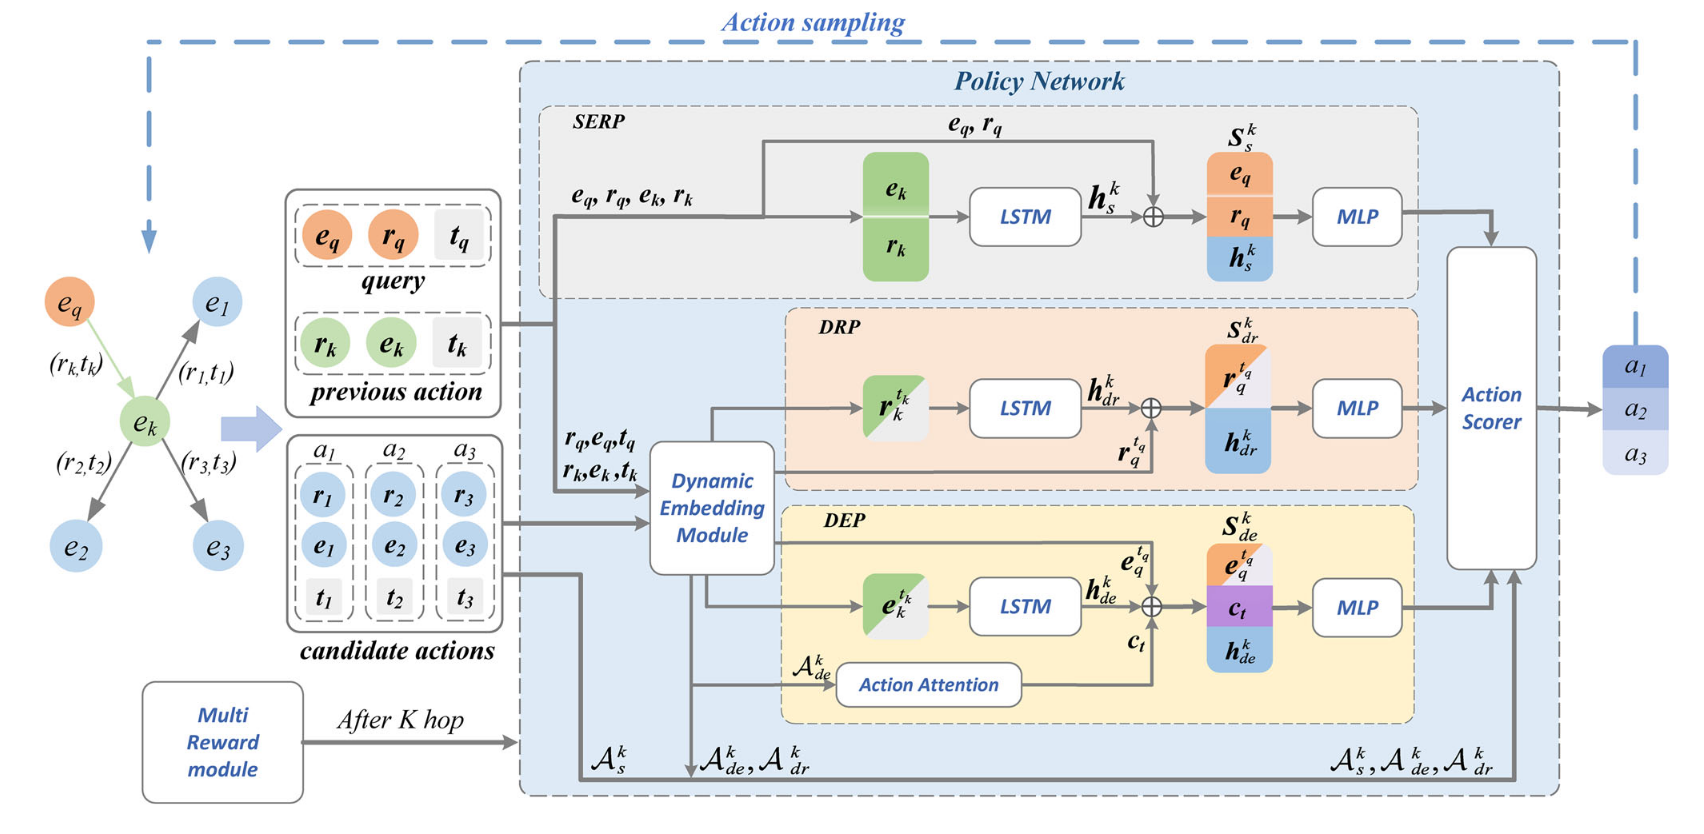
\includegraphics[width=1.0\textwidth]{figures/MPNet.png}
	\caption{MPNet 的整体框架结构,其 SERP、DRP和DEP 三种策略网络使用各自的LSTM模块分别记录之前动作的静态信息、动态实体信息和动态关系信息\cite{4-2024}。}
\end{figure}



\subsection{简介}

强化学习把预测任务视为一个马尔可夫决策过程(Markov Decision Process,MDP),MPNet 采用了与 TLogic 相似的表示方法,并且也引入了逆关系这一表示,它的核心组件是策略网络和奖励机制。策略网络包括三种:SERP 对基于实体和关系的静态特征的行为进行打分;DRP 和 DEP 分别对实体和关系的动态特征所执行的动作进行打分。

实体和关系的动态特征是通过动态嵌入模块获得的,其中 DEP 使用注意力机制来聚合候选动态实体的信息并将其作为模型状态的一部分,这么做有助于让代理关注于高价值的实体。每一个候选动作的分数结合了三个策略的输出结果,然后通过一个候选动作的动作打分模块计算得来;之后再根据所到分数按概率来选择候选行为。经过有限次跳跃之后,奖励机制根据代理的位置来计算给出的奖励,整个模型以获得最高奖励分数为训练目标。


\subsection{定义与形式化表达}

逆边:对每个四元组 $(e_s,r,e_o,t)$ 构建一个逆向关系四元组 $(e_o,r^{-1},e_s,t)$ ;

自循环边:是指代理可以在某一次跳跃中保持原来的位置不变,这可以作为代理抵达目标的判断依据;

时序边:如果代理在 $t_i$ 时刻位于 $e_i$,如果存在一条路径 $(e_i,r,e_j,t_j)$ 其中 $t_i\le t_j<t_q$,其中 $t_q$ 表示查询目标的时间,这样构建的边称为时序边;

回溯边:如果代理在 $t_i$ 时刻位于 $e_i$,如果存在一条路径 $(e_i,r,e_j,t_j)$ 其中 $t_i< t_j<t_q$,其中 $t_q$ 表示查询目标的时间,这样构建的边称为回溯边;

关系相关边:对于查询 $(e_s,r_q,?,t_q)$,如果 $e_s$ 是一个未见实体,可以使用关系相关边来定位在过去的时刻中具有关系 $r_q$ 的所有事实。比如,如果存在 $(e_i,r_q,e_j,t_k)$ ,且有 $t_k<t_q$,那么这条边就可以被构建,它就是一个关系相关边。利用关系相关边,对于未见实体仍然可以从历史中探索答案。

${\mathcal S}$ 用来表示状态,${\mathcal S}=\{{\mathcal H},{\mathcal Q}\}$,其中 ${\mathcal H}$ 表示代理已经探索过的信息,${\mathcal Q}$ 代表当前查询的信息。代理收到查询后,其初始状态记为 ${\mathcal S}^0=\{{\mathcal H}^0,{\mathcal Q}\}$;特别地,对于动态实体策略,初始状态表示为 ${\mathcal S}^0_{de}=\{{\mathcal H}^0_{de},{\mathcal C},{\mathcal Q}\}$,其中 ${\mathcal C}$ 表示使用注意力机制的当前候选动作的表征。

${\mathcal A}$ 用于表示动作空间的集合,如果代理的当前实体 $e_i^{t_i}$ 已知,$e_i$ 在第 $k$ 步的动作空间 ${\mathcal A}^k$ 可以记为${\mathcal A}^k_{seen}=\{(r’,e’,t’)|(e_i,r’,e’,t’)\in{\mathcal F}\}$;相反,若 $e_i$ 未知,相应的动作空间记为:${\mathcal A}^k_{unseen}=\{(r_q,e’,t’)|(e_i,r_q,e’,t’)\in{\mathcal F}\}$。

状态转换函数记为 $\delta:{\mathcal S}\times{\mathcal A}\rightarrow{\mathcal S}$ ,特别地,${\mathcal S}^{k+1}=\delta({\mathcal S}^k,{\mathcal A}^k)$ 。

强化学习最基本的奖励策略就是看代理是否抵达了目标实体。在达到限定跳数之后,如果代理抵达了目标实体,奖励为1,否则奖励为0,表达为:${\mathcal R}({\mathcal S}^K)={{\mathbb I}\{e_K=e_{target}\}}$。


\subsection{策略网络}

SERP 部分不考虑时间,当代理执行了 $k$ 步之后,使用一 LSTM 来捕获历史路径,表达如下:

\begin{equation}
	\begin{aligned}
h^k_s & =\text{LSTM}(h_s^{k-1},[r_k\oplus e_k]) \\ 
h^0_s & =\text{LSTM}(0,[r_{loop}\oplus e_q])
	\end{aligned}
\end{equation}

其中 $\oplus$ 表示连接操作,$h_s^k\in{\mathbb R}^{d_n}$ 第 $k$ 步的历史信息,此时的状态记为$S_s^k=[e_q\oplus r_q \oplus h^k_s]$, $S_s^k\in{\mathbb R}^{d_e+d_r+d_h}$,$d_e,d_r,d_h$ 分别表示实体、关系与历史信息的词嵌入维度。状态 $s_s^k$ 随后输入到一个两层的 MLP 中进行编码,然后用如下函数为候选动作进行打分:

\begin{equation}
\varphi_s(a_i|S^k_s)={\mathcal A}_s^k W_{s2}\text{ReLU}(dropout(W_{s1}S^k_s))
\end{equation}

其中 $W_{s1},W_{s2}$ 是可学习的线性转换矩阵。

在动态实体策略 DEP 中,时间编码器的形式化表达如下:

\begin{equation}
	\begin{aligned}
e_k^{t_k} & =(e_k\oplus\phi(\Delta t_k)) \\ 
\phi(\Delta t_k) & =\sin({\boldsymbol w}_s\Delta t_k+{\boldsymbol b}_s)+\tanh({\boldsymbol w}_t\Delta t_k+{\boldsymbol b}_t)
	\end{aligned}
\end{equation}

其中 ${\boldsymbol w}_s,{\boldsymbol b}_s,{\boldsymbol w}_t,{\boldsymbol b}_t$ 可以学习的参数向量。

与 SERP 类似,在 $k$ 步之后,DEP 使用 LSTM 来记录动态实体的历史路径:

\begin{equation}
	\begin{aligned}
h^k_{de} & =\text{LSTM}(h_{de}^{k-1},e_k^{t_k}), \\ 
h^0_{de} & =\text{LSTM}(0,e_q^{t_q})
	\end{aligned}
\end{equation}

为了方便代理选择下一步动作,DEP 使用注意力机制来为每一个候选动作设定注意力分数,动态候选实体可表示为:

\begin{equation}
{\bold C}^k_{de}=({\mathcal A}^k_{de}W_1)\text{Softmax}\left(({\mathcal A}^k_{de}W_2)^T({\mathcal A}^k_{de}W_3)\right)
\end{equation}

从而有 $S_{de}^k=[e_q^{t_q}\oplus c_t \oplus h^k_{de}]$,动态实体的候选分数计算方法为:

\begin{equation}
\varphi_{de}(a_i|S^k_{de})={\mathcal A}_{de}^k W_{de2}\text{ReLU}(dropout(W_{de1}S^k_{de}))
\end{equation}

与DEP类似,DRP的嵌入表示可表达为 $r_k^{t_k}=(r_k\oplus\phi(\Delta t_k))$,同样的有:

\begin{equation}
	\begin{aligned}
h^k_{dr} & =\text{LSTM}(h_{dr}^{k-1},r_k^{t_k}) \\ 
h^0_{dr} & =\text{LSTM}(0,r_{loop}^{t_q})
	\end{aligned}
\end{equation}

以及 $S_{dr}^k=[r_q^{t_q}\oplus h^k_{dr}]$,分数计算函数为:

\begin{equation}
\varphi_{dr}(a_i|S^k_{dr})={\mathcal A}_{dr}^k W_{dr2}\text{ReLU}(dropout(W_{dr1}S^k_{dr}))
\end{equation}


\subsection{多重奖励机制及优化}

MPNet 的奖励由三部分构成:全局奖励 $r_g$、基于频率的奖励 $r_f$,效率奖励 $r_e$,最终奖励为:

\begin{equation}
R=(1+\alpha_1 r_f)(r_g+\alpha_2 r_p)
\end{equation}

对每次 $K$ 步操作,策略序列记为 $\pi_{\theta}=\{a_1,a_2,\dots,a_K\}$,目标函数定义如下:

\begin{equation}
\begin{aligned}
	\begin{split}
		J(\theta)= & {\mathbb E}_{e_q,r_q,e_{target},t_q}\sim{\mathcal F}_{train}\\
		& [{\mathbb E}_{a_1,a_2,\dots,a_K\sim\pi_{\theta}}[R(S^K|e_q,r_q,t_q)]]
	\end{split}
\end{aligned}
\end{equation}

然后使用策略梯度方法进行优化,对 $\theta$ 进行更新。

\subsection{实验结果}

MP-Net 在实验中的表现如下:




\begin{table}[htbp]
	\centering
	\caption{MP-Net 在 icews14 上的表现}
	\begin{tabular}{cccc}
		\toprule  % 顶部线
		MMR&Hit@1&Hit@3&Hit@10 \\ 
		\midrule  % 中部线
		0.4376&0.3485&0.4823&0.6061 \\
		\bottomrule  % 底部线
	\end{tabular}
\end{table}






\section{基于 Transformer 的方法:ECEformer}



\begin{figure}
	\captionsetup{width=0.85\textwidth}
	\centering
	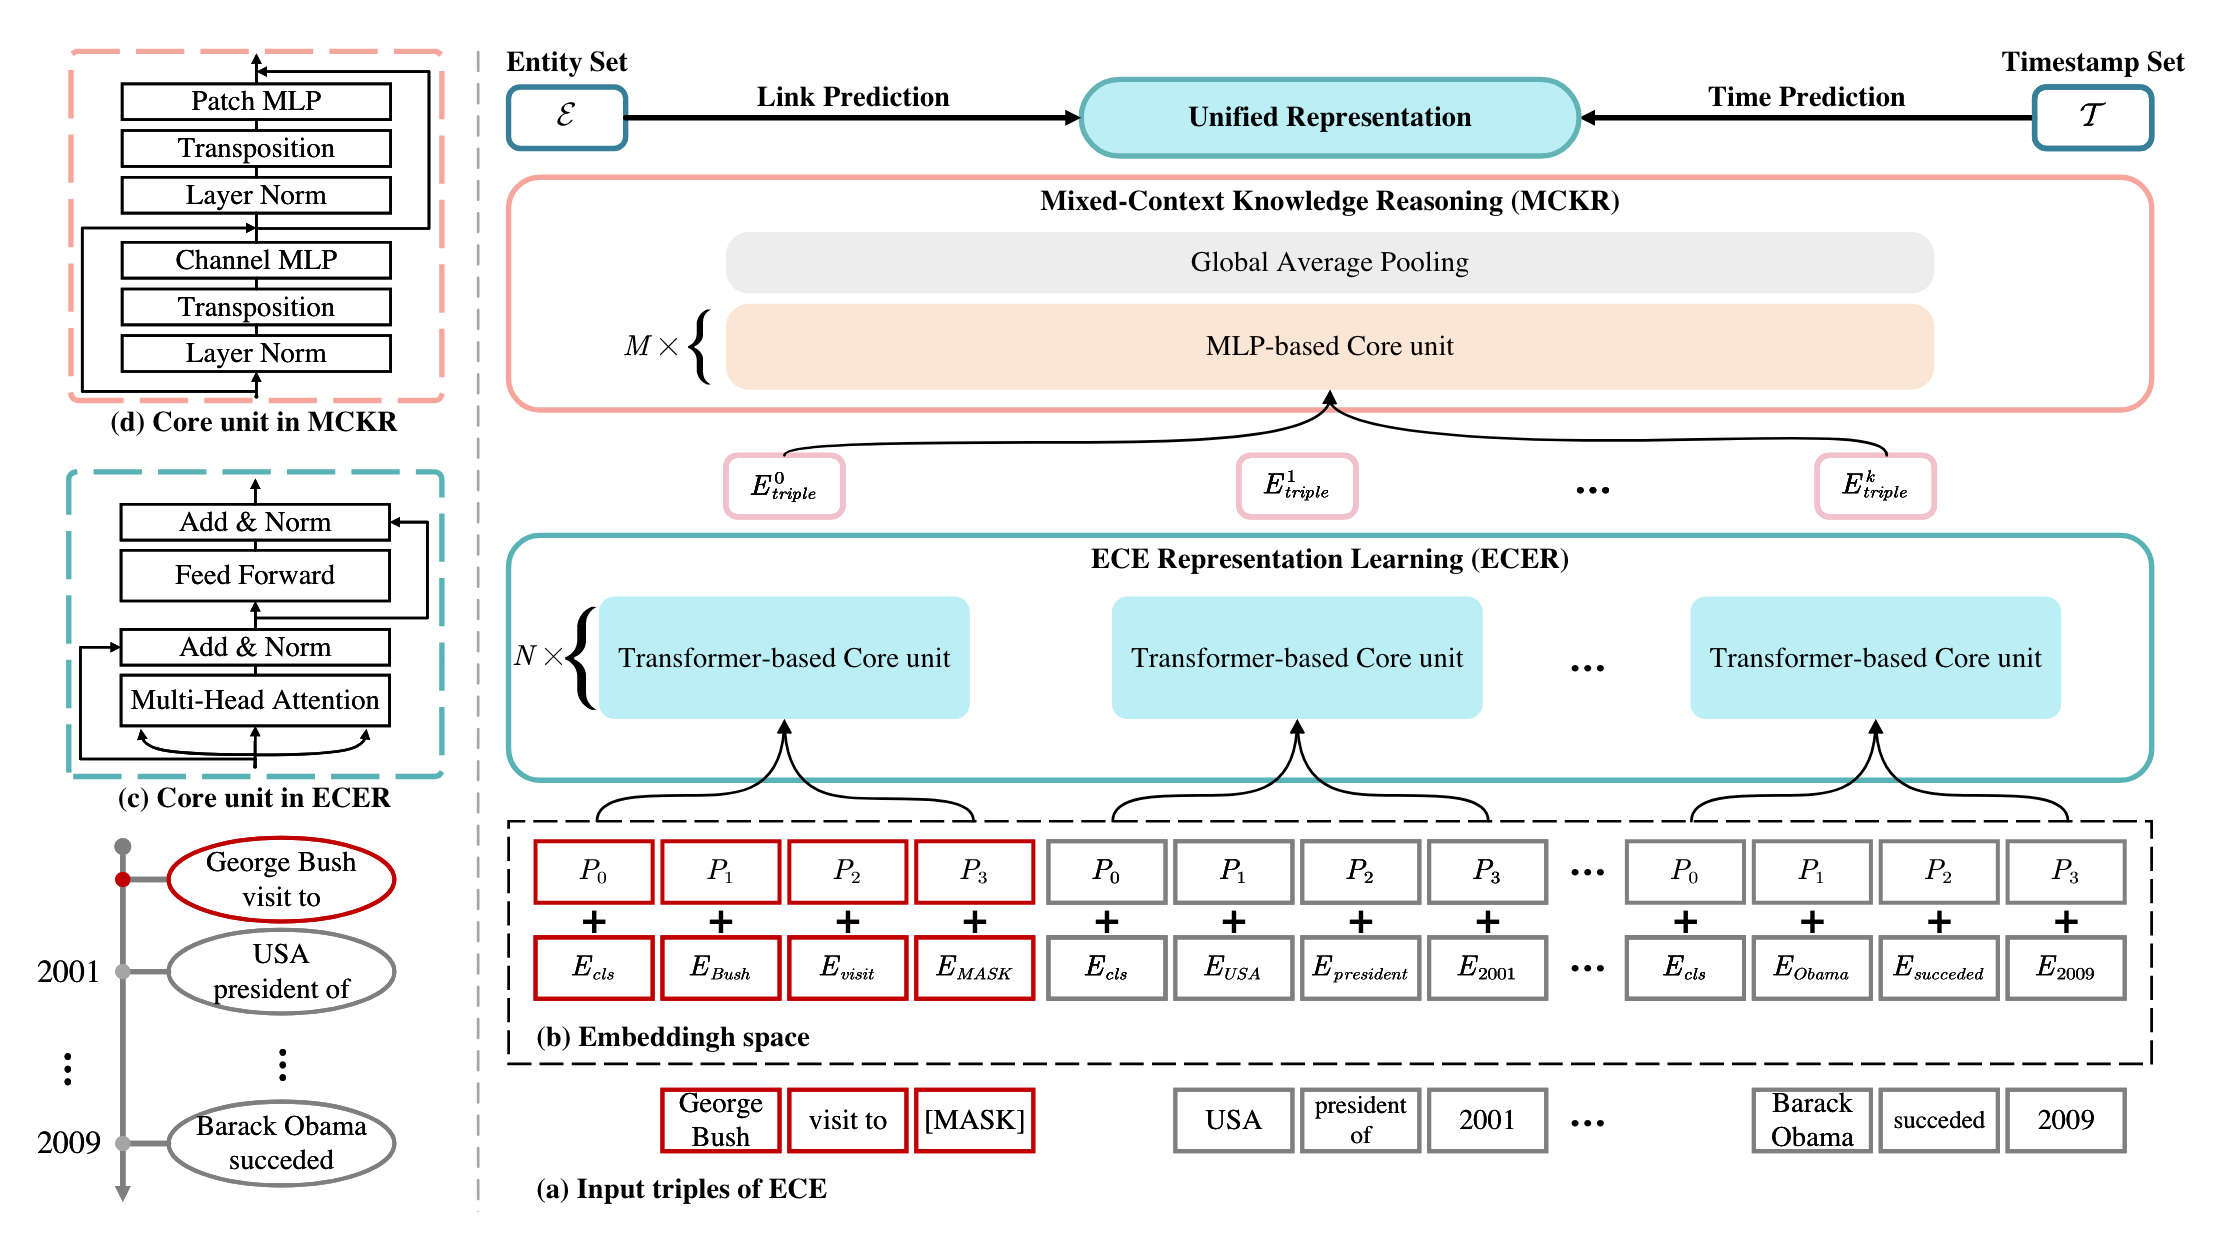
\includegraphics[width=1.0\textwidth]{figures/ECEformer.png}
	\caption{ECEformer 的整体结构\cite{6-2024}。ECER 和 MCKR 是其核心组件。}
	\label{fig:enter-label}
\end{figure}



\subsection{简介}

ECE 表示事件进化链,它用于把与指定请求的邻居子图相关的结构与时序上下文转化为一种结构化的知识序列。具体来说,对于请求 $(s,p,?,\tau)$ ,ECE 被概念化为一个单链表 ${\mathcal C}=\{C_0,C_1,\dots,C_k\}$ ,其中 $C_i$ 表示与 $s$ 相关的事件,可以表达为 $(e,p,\tau)$,其中的 $e$ 既可以是头实体也可以是尾实体。这样 $C_0$ 表示就是请求自身,而 $C_k$ 则表示邻接事件,$k$ 用于限制邻接事件的数量。这样 ECE 就既可以得到四元组内部的结构信息,也可以得到四元组之间的结构信息。
ECEformer 主要由两个模块组成:ECE 表示学习(ECER)和混合上下文知识推理(MCKR)。前者 ECER 用来探索图中的结构与语义关系,后者 MCKR 用来发掘与查询相关的历史信息,即学习不同四元组之间上下文与时间相关性的统一表示。


\subsection{方法实现}

ECER由 N 个核心单元组成,每一个核心单元都由多头注意力层(MHA)、归一化层(LN)和基于 MLP 的前馈(FF)交替构成。其中 MHA 和 FF 都通向一个带残差连接(RC)的 LN;FF 层由两个带 GELU 非线性激活函数的层组成。此过程可表达为:

\begin{equation}
y=l\circ r\circ f\circ l\circ r \circ h(x;W_h,W_l,W_f)
\end{equation}

其中 $h$ 表示带权重 $W_h$ 的 MHA 函数,$l$ 表示带权重 $W_l$ 的 LN 函数,$f$ 表示带权重 $W_f$ 的 FF 函数;

$r$ 表示 RC 函数, $x$ 表示输入序列,$y$ 表示输出的词嵌入,$\circ$ 是合成函数算子。

MHA 靠尺度化的点积注意力机制来学习当前 token 和序列中所有 tokens 之间的语义交互,从而全面地探索每个事件中的结构与语义信息。直接将时间作为 token 输入 ECER 也使得它可以从每个事件中通过语义来提取时序信息。

对于一个请求 $(s,p,?,\tau)$ 以及它对应的 ECE $C_q$,其分支中的每一个成分被视作一个 token,并按时间顺序展开整个链。通过增加一些特殊 token,所有元素(token)被编码为语义嵌入 $E$ 和位置嵌入 $P$ ,两者拼接后作为 token 的表示。表达如下:

\begin{equation}
E^i_{inp}=E_i+P_j,\{i\in{\mathcal E}\cup{\mathcal R}\cup{\mathcal T},j\in[0,1,2,3]\}
\end{equation}

其中 $E^i_{inp}$ 表示输入序列的第 $i\text{-th}$ token,$E_i$ 表示特征嵌入,$P_i$ 表示位置嵌入。这些嵌入交替输入到 ${\mathcal F}_ECER:{\mathbb R}^{4\times d}\rightarrow {\mathbb R}^d$ *,*最终输出由 $E^i{triple},i=0,1,\dots,k$ 表示,其中既有语义信息,又有位置信息。


MCKR 的输入是 $k+1$ 个嵌入表示,形成一个二维的真值输入矩阵 ${\mathcal M}\in{\mathbb R}^{(1+k)\times d}$ 。它包含 $M$ 个核心单元,每一个核心单元由两个关键混合层组成:MLP 通道和 MLP 补丁。另外,每个混合单元都会被一个归一化层和转化层执行后续处理。

MLP 通道以 ${\mathcal M}$ 的一列作为输入,映射后不改变列的维度 $k+1$;它的目的是在同一个特征维度上促进跨事件嵌入的信息交互。MLP 补丁作用于 ${\mathcal M}$ 的行,映射不改变行的维度 $d$;它的目标是在同一个事件嵌入里促进不同特征维度间的信息交互。这个过程可以表达为:

\begin{equation}
\dot{\mathcal M}_{\*,i}=M_{\*,i}+W_2\sigma(W_1\text{Norm}({\mathcal M})_{\*,i}),\ \text{for}\ i=1,2,\dots,d
\end{equation}

\begin{equation}
\ddot{\mathcal M}_{j,\*}=\dot{\mathcal M}_{j,\*}+W_4\sigma(W_3\text{Norm}(\dot{\mathcal M})_{j,\*}),\ \text{for}\ i=1,2,\dots,k+1
\end{equation}

其中 $\sigma$ 是非线性激活函数 GELU。$W_1,W_2$,$W_3,W_4$ 分别是 MLP 通道和 MLP 补丁里的隐权重。

借鉴了 Mlp-mixer 中的方法,MCKR 使用同样的参数来“翻译”两个核心 MLP 单元中的列或者行,这种参数共享机制使得网络具有了位置不变性,增强了其熟练处理序列数据的能力。而且这种方法还可以规避随着维度扩张而增加的模型复杂度。

之后是一个全局的平均池化层,它可以对混合上下文 $\ddot{M}$ 进行蒸馏:

\begin{equation}
{\mathcal U}_{ECE}=\text{GlobalAvgPool}(\ddot{M})
\end{equation}

其中 ${\mathcal U}_{ECE}$ 表示 ECE 的统一表示。对于一个没有头实体或者没有尾实体的四元组,链路预测任务可以通过计算 ${\mathcal U}_{ECE}$ 与所有候选实体之间的相似性来获得,表达为数学形式如下:

\begin{equation}
p(e_{gt}|q)=Softmax(Sim(\mathcal{U}_{ECE},\mathcal{E}))
\end{equation}

其中 $Sim$ 是 $\mathcal{U}_{ECE}$ 和候选实体之间的相似函数,$q$ 表示预测结果,基于相似分数选择 $top\text{-}1$ 的实体得到;$p(e_{gt}|q)$ 表示 $q$ 是目标实体 $e_{gt}$ 时的概率。


\subsection{时间信息强化任务与优化}

如果事件经常与某个特定的时间点一同出现,通过链路预测学到的统一表示并不是通过上下文信息得到的解。这样的表示会引入虚假的相关性,因为它只考虑了实体与关系而无视了事件的时间。

文章通过一个标记时间预测任务来强化在语境化过程中对时间信息的探索,它在 ECE 的特定请求分支中使用一个特殊的 token $[MASK]$ 来替换时间 $\tau$ 。这个设计可以鼓励模型同化上下文信息并对特定的请求事件演绎其发生时间,这个方法与链路预测其实是一类似的,只不过链路预测预测的是实体。

对链路预测和时间预测,ECEformer 都使用交叉熵函数来计算损失;为了让模型适应不同的训练集并降低内存使用,文章还引入了一个类似于 edge dropout regularization 的 ECE 采样策略,它只采样查询对象的部分邻居信息,并把 ground truth 目标实体从采样到的信息中剔除。


\subsection{实验结果}

ECEformer 在实验中的表现如下:




\begin{table}[htbp]
	\centering
	\caption{MP-Net 在 icews14 上的表现}
	\begin{tabular}{cccc}
		\toprule  % 顶部线
		MMR&Hit@1&Hit@3&Hit@10 \\ 
		\midrule  % 中部线
		0.7170&0.6731&0.7360&0.8030 \\
		\bottomrule  % 底部线
	\end{tabular}
\end{table}






\section{总结}

在上述算法中我们可以看到,有些方法并不会局限于其核心方法,会适当地引入其它算法。比如在强化学习框架 MP-Net 中的编码步骤就使用了注意力机制。基于人工神经网络的方法一直被人诟病存在不可解释性以及幻觉问题,而基于规则的方法可以有效弥补这一点,如果能把两者结合在一起是一个值得考虑的研究方向。



% 参考文献 %
\bibliographystyle{IEEEtran}
\bibliography{cite}

\end{document}
